\documentclass{article}
\usepackage{amsmath}
\usepackage[utf8]{inputenc}
\usepackage{float}
\usepackage{epsfig,graphicx}
\usepackage{xcolor,import}
\usepackage[german]{babel}
\usepackage{textcomp}
\usepackage{mathtools}

\begin{document}
\thispagestyle{empty}
			\begin{center}
			\Large{Fakultät für Physik}\\
			\end{center}
\begin{verbatim}


\end{verbatim}
							%Eintrag des Wintersemesters
			\begin{center}
			\textbf{\LARGE WINTERSEMESTER 2014/15}
			\end{center}
\begin{verbatim}


\end{verbatim}
			\begin{center}
			\textbf{\LARGE{Physikalisches Praktikum 1}}
			\end{center}
\begin{verbatim}




\end{verbatim}

			\begin{center}
			\textbf{\LARGE{PROTOKOLL}}
			\end{center}
			
\begin{verbatim}





\end{verbatim}

			\begin{flushleft}
			\textbf{\Large{Experiment Nr.9:} Gleichstrom}\\
							%Experiment Nr. und Titel statt den Punkten eintragen
			\LARGE{}	
			\end{flushleft}

\begin{verbatim}

\end{verbatim}	
							%Eintragen des Abgabedatums, oder des Erstelldatums des Protokolls
			\begin{flushleft}
			\textbf{\Large{Datum:}} \Large{12.12.2014}
			\end{flushleft}
			
\begin{verbatim}
\end{verbatim}
							%Namen der Protokollschreiber
		\begin{flushleft}
			\textbf{\Large{Namen:}} \Large{Veronika Bachleitner, Erik Grafendorfer}
			\end{flushleft}

\begin{verbatim}


\end{verbatim}
							%Kurstag und Gruppennummer, zb. Fr/5
			\begin{flushleft}
			\textbf{\Large{Kurstag/Gruppe:}} \Large{Fr/1}
			\end{flushleft}

\begin{verbatim}






\end{verbatim}
							%Name des Betreuers, das Praktikum betreute.
			\begin{flushleft}
			\LARGE{\textbf{Betreuer:}}	\Large{}	
			\end{flushleft}
\newpage	

\section{Photovoltaische Solarzellen als Gleichstromquelle}

\subsection{Aufgabenstellung}
\subsection{Grundlagen}
\subsection{Versuchsaufbau und Methoden}
\subsection{Durchführung}
\subsection{Ergebnisse}
RL 1kOhm +- 5%, +- 0.25% Lin
RI 0.517 Ohm

\subsection{Diskussion}

\section{Widerstandsbestimmung mittels Wheatstone Brücke}

\subsection{Aufgabenstellung}
Wir messen drei unbekannte Widerstände mit Hilfe einer Brückenschaltung.
Außerdem messen wir den Gesamtwiderstand zweier Widerstände einmal in einer Reihenschaltung und einmal in einer Parallelschaltung und vergleichen unsere Messungen mit berechneten Ergebnissen.
\subsection{Grundlagen}
\subsection{Versuchsaufbau und Methoden}
\subsection{Durchführung}
\subsection{Ergebnisse}
Testwiderstand R0: 1kOhm
\subsection{Diskussion}

\section{Reale Spannungsquelle}

\subsection{Aufgabenstellung}
Wir nehmen die Strom-Spannungskennlinie einer Batterie auf und bestimmen daraus den Innenwiderstand der Batterie und die Quellenspannung.


\subsection{Grundlagen}
Eine reale Spannungsquelle hat einen endlichen Innenwiderstand. Um das Verhalten der Quelle in einem Stromkreis trotzdem beschreiben zu können, müssen wir iein Ersatzschaltbild machen: Mit einer idealen Quelle, die also keinen Innenwiderstand besitzt, und einen dazu in Serie geschaltenen Widerstand $R_i$.\\
Die Quellenspannung ist die Spannung der idealen Batterie.\\
Der Strom $I=U_0/(R_i+R_L)$ bewirkt einen Spannungsabfall am Innenwiderstand, daher bezeichnen wir die Spannung der realen Batterie (Klemmenspannung): $U_{KL}=U_0-IR_i$.


\subsection{Versuchsaufbau und Methoden}
Aus den Grundlagen finden wir eine Methode, den gesuchten Innenwiderstand der Batterie zu bestimmen:\\
Wir messen die Klemmenspannung als Funktion des Stromes: $U_{KL}=U_{KL}(I)$. Die Steigung der resultierenden Gerade ist gleich $R_i$.\\
Weiters kann die Quellenspannung $U_0$ durch Extrapolation bestimmt werden.\\
\\
Wir verwenden eine Batterie, ein Volt- und ein Ampèremeter (beides Fluke 183), eine Widerstandsdekade als Lastwiderstand und einen Taster zum Öffnen/Schließen des Stromkreises.\\
\\
\textbf{Unsicherheiten der Messgeräte:} \\
Ampèremeter - Fluke 183:\\
Auflösung: $100\mu A$\\
Genauigkeit: $\pm$ (0,2\% + 4 Zählimpulse)\\
\\
Voltmeter - Fluke 183:\\
Auflösung: $1mV$\\
Genauigkeit: $\pm$ (0.07\% + 1 Zählimpuls)


\subsection{Durchführung}
Wir messen die Leerlaufspannung mit offenem Taster. Sie verändert sich während unserer Messung vernachlässigbar; um 0.001V.\\ 
Anschließend messen wir $U_{KL}$ und $I$ mit variablen Widerständen. Wir gehen dabei in Schritten von $20\Omega$ von 200$\Omega$ bis $20\Omega$.\\
Die Daten werten wir mit QTI-Plot aus.

\newpage
\subsection{Ergebnisse}
Leerlaufspannung: 1.505V\\
\\


\begin{tabular}{|r|l|l|}
\hline
$R_L$ $[\Omega]$ & Spannung U [V] & Strom I [mA]\\
\hline
200 & 1.494 $\pm$ 0.002 & 7.43 $\pm$ 0.055\\
180 & 1.494 $\pm$ 0.002 & 8.26 $\pm$ 0.057\\
160 & 1.492 $\pm$ 0.002 & 9.27 $\pm$ 0.059\\
140 & 1.491 $\pm$ 0.002 & 10.59 $\pm$ 0.062\\
120 & 1.489 $\pm$ 0.002 & 12.32 $\pm$ 0.065\\
100 & 1.487 $\pm$ 0.002 & 14.73 $\pm$ 0.070\\
80 & 1.483 $\pm$ 0.002 & 18.33 $\pm$ 0.077\\
60 & 1.477 $\pm$ 0.002 & 24.27 $\pm$ 0.089\\
40 & 1.466 $\pm$ 0.002 & 35.94 $\pm$ 0.12\\
20 & 1.445 $\pm$ 0.002 & 69.20 $\pm$ 0.18\\
\hline
\end{tabular}


\begin{center}
\begin{figure}[H]
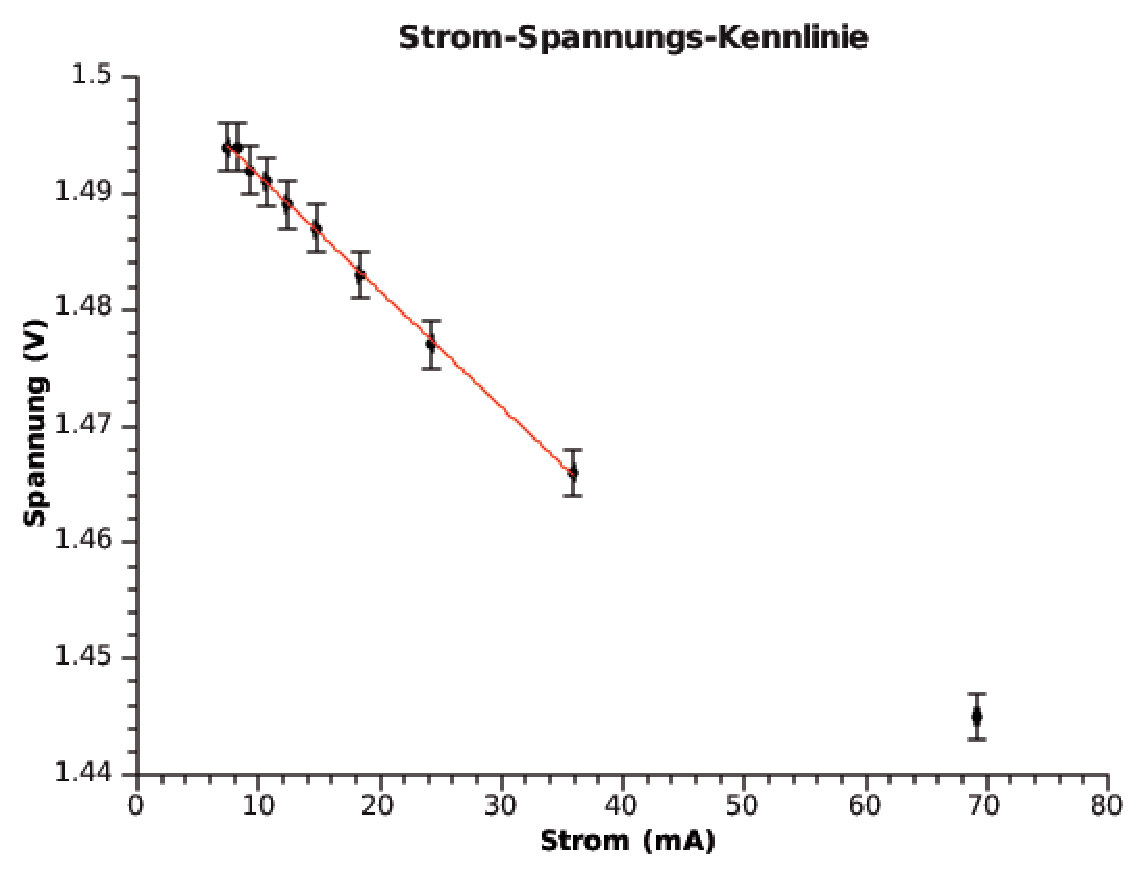
\includegraphics[scale=0.5]{batterie_kennlinie.eps} 
\end{figure}
\end{center}

QTI-Plot gibt uns für den Fit mittels $y=Ax+B$ (wobei y: Spannung U, x: Strom I) die folgenden Werte: 
\begin{quote}
From $x = 7.43$ to $x = 35.94$\\
$a  = -0.000995923244694066 \pm 1.39673189659993e-05$\\
$b  = 1.50150717852846 \pm 0.000251022348126121$\\
-------------------------------------\\
$R^2 = 0.998625088078122$\\
\end{quote}


\newpage
Unser Ergebnis für den Innenwiderstand der Batterie ist der Wert der Variable a mal 1000. (Da wir für den Strom mA verwendet haben.)\\
$$\boxed{R_i=(0.996 \pm 0.014)\Omega}$$\\
\\
Unser Ergebnis für die Quellenspannung ist der Wert der Variable b. \\
$$\boxed{U_0=1.50151 \pm 0.00026}$$


\subsection{Diskussion}
\textbf{Eine Anmerkung zu unseren Unsicherheiten:}\\
Bei der Strommessung ist uns aufgefallen, dass bei einigen Werten die Unsicherheit mit der Rundung auf 2 relevante Stellen eine Nachkommastelle mehr besitzt als unser eigentlicher Wert.\\
Wir überprüfen also, ob eine Rundung auf eine Stelle weniger sinnvoll ist. Dies taten wir nach Anleitung aus der Vorlesung "Auswertung und Dokumentation experimenteller Daten" und sehen daraus, dass wir eine zusätzliche Rundungssicherheit von 11\% im Maximum erhalten würden. Daher belassen wir die Unsicherheiten wie sie sind.\\
\\
\textbf{Zu den Ergebnissen:}\\
Wir ignorieren den Wert $I=69.20$ bei der Erstellung der Stroms-Spannungs-Kennlinie, da dieser den linearen Fit hebelt. Der Wert ist beinahe doppelt so groß wie der vorhergehende. Wir erklären uns dies dadurch, dass der Widerstand hier schon sehr klein ist und wir uns bei den $20\Omega$ schon nahe am Kurzschluss befanden.
\\
Das Ergebnis für den Innenwiderstand $R_i\approx 1\Omega$ ist laut unserem Betreuer passend.\\
Die Quellenspannung entspricht wie erwartet etwa der gemessenen Leerlaufspannung.

\newpage

\section{Belasteter Spannungsteiler}

\subsection{Aufgabenstellung}
\subsection{Grundlagen}
\subsection{Versuchsaufbau und Methoden}
\subsection{Durchführung}
\subsection{Ergebnisse}
\subsection{Diskussion}
\end{document}
